\documentclass[a4paper]{article}
\usepackage[margin=3cm]{geometry}
\usepackage{xcolor}
\usepackage{graphicx}
\usepackage{lipsum}
\usepackage{amsmath}
\usepackage{pdfpages}
\usepackage{url}
\usepackage{hyperref}
\usepackage{subcaption}
\usepackage{siunitx}
\hypersetup{
	colorlinks = true,
	colorlinks = false,
	linkbordercolor = {white},
	urlcolor = {blue},
	linkcolor = {blue},
	citecolor = {blue}
}
\usepackage{acronym}
\usepackage[acronym,nomain]{glossaries}
\makeglossaries
\newcommand{\todo}[1]{\textbf{\textcolor{red}{#1}}}
\newcommand{\td}[1]{\textbf{\textcolor{red}{#1}}}
\newcommand{\me}[1]{\textcolor{gray}{#1}}
\newcommand{\ds}[1]{}
\newcommand{\x}{$\times$}
\newcommand{\picwidth}{0.7\textwidth}

%SI UNITS
\newcommand{\cm}[1]{\SI{#1}{\centi\meter}}
\newcommand{\mm}[1]{\SI{#1}{\milli\meter}}
\newcommand{\mg}[1]{\SI{#1}{\milli\gram}}
\newcommand{\ml}[1]{\SI{#1}{\milli\liter}}
\newcommand{\um}[1]{\SI{#1}{\micro\meter}}
\newcommand{\ul}[1]{\SI{#1}{\micro\liter}}
\newcommand{\minutes}[1]{\SI{#1}{\minute}}
\newcommand{\oc}[1]{\SI{#1}{\degreeCelsius}}
\newcommand{\s}[1]{\SI{#1}{\second}}
\newcommand{\h}[1]{\SI{#1}{\hour}}

\title{Functional oxide layers for electrical isolation and chemical passivation of steel substrates}
\author{Johann Dorn}

\begin{document}
\maketitle
\newacronym{zrpro}{Zr(PrO)$_4$}{zirconium(IV)propoxide}
\newacronym{acac}{Hacac}{acetylacetone}
\newacronym{acoh}{AcOH}{acetic acid}
\newacronym{buoh}{BuOH}{1-buthanol}
\newacronym{ipo}{IPO}{2-Propanol}
\newacronym{ito}{ITO}{indium doped tin oxide}
\newacronym{fto}{FTO}{fluorine doped tin oxide}
\newacronym{n2}{N$_2$}{nitrogen}
\newacronym{water}{H$_2$O}{deionized water}
\newacronym{sds}{SDS}{sodium dodecyl sulfate}
\newacronym{hcl}{HCl}{hydrochloric acid}
\newacronym{h2so4}{H$_2$SO$_4$}{sulfuric acid}
\newacronym{naoh}{NaOH}{sodium hydroxide}
\newacronym{zro}{ZrO$_2$}{zirconium dioxide}
\newacronym{1f}{1F}{one-fold concentrated solution}
\newacronym{2f}{2F}{two-fold concentrated solution}
\newacronym{3f}{3F}{three-fold concentrated solution}
\newacronym{4f}{4F}{four-fold concentrated solution}
\newacronym{5f}{5F}{five-fold concentrated solution}
\newacronym{db}{DB}{doctor blading}
\newacronym{pv}{PV}{photovoltaic}
\newacronym{cigs}{CIGS}{copper indium gallium sulfide}
\newacronym{sg}{SG}{sol-gel}

\clearpage
\section*{Abstract}
%\lipsum[1]
\td{A thin zirconium oxide layer was aufgetragen via doctor blading on a steel foil substrate with the goal of erhalten an moeglichst homogenuous and insulating layer.
The layers were characterized over the current-voltage curve and the operational variables were optimized with an pso swarm optimization algorithm.
}
\section*{Preface}
\lipsum[2]
%Thank
%I want to thank Theodoros Dimopulos, Adhi, Neha, Philipp. 
%Quyhn, Maria, Jana, Vivien and Katharina who tried to keep me sane throughout the
%Elif 
\clearpage
\tableofcontents
\clearpage
\printglossaries
\clearpage
%%%%%%%%%
%%%%%%%%%%%%%%%%%%%%%%%%%%%
%%%%%%%%%%%%%%%%%%%%%%%%%%%%%%%%%%%%%%%%%%%%%%%%%%%%%%

%%%%%%%%%
%%%%%%%%%%%%%%%%%%%%%%%%%%%
%%%%%%%%%%%%%%%%%%%%%%%%%%%%%%%%%%%%%%%%%%%%%%%%%%%%%%
\section{Introduction}
\td{describe everything what is mentioned in \ref{sec:exp}}
\Gls{pv} is one big hope when trying to become carbon neutral as it uses the energy provided by sun directly in contrast to renewable energy sources (e.g. wind and water) or even carbon based sources.
One sort of \gls{pv} are \gls{cigs} \cite{Vasekar2010} cells. % https://doi.org/10.1016/j.tsf.2009.09.033}
In order to make a module, multiple cells are operated in series. 
The cells must be applied to a non-conducting surface.
Glass is a good non-conducting substrate, but very rigid and brittle. 
An alternative is steel, which is ductile, inexpensive and highly available, but conducting. 
An insulating layer must therefore be applied to the steel substrate before any \gls{cigs} cells can be applied.
A non-toxic material which is suitable for this application is \gls{zro}. 
An economic and scalable method is doctor blading via a \gls{sg} process. 
\gls{sg} processes often produce porous layers. 
In this work a dense, insulating and homogeneous layer is pursued. 
ML can help to uncover complex non-linear relations, such as the influence of the production factors on the thickness and resistance of the resulting layer.
The minisation of the conductance if performed with a particle swarm optimization algorithm.
%%%%%%%%%
%%%%%%%%%%%%%%%%%%%%%%%%%%%
%%%%%%%%%%%%%%%%%%%%%%%%%%%%%%%%%%%%%%%%%%%%%%%%%%%%%%
\section{Aims and Objectives}
The aim of this work is to develop a non-conducting layer on steel based on  non-toxic materials like Aluminium or Zirconium via doctor blading. 
This layer can then be used as insulator for CIGS modules on steel sheets.
Doctor blading - or tape casting - is a widely used precision coating method to apply thin films on large area surfaces\cite{Berni2004}.
%The method of doctor blading, which is in principle a sol-gel process, 
This sol-gel process was chosen because of the availability to the industrial partner.
In order to optimize the resulting layer the multitude of parameters was optimized with an particle swarm optimization ansatz. %machine learning 
The conductivity (dependent variable), the number of layers and calcination time (both independent variables) should be minimized.
%The conductivity should be as small as possible.
%The number of layers should be held small and the calcination heating rate should be maximized. 
\iffalse
Defensio: Argumente in der Arbeit noch mal sichten, Feedback von Betreuungsperson im Kopf haben - da könnten Fragen kommen, 
sich selbst aufnehmen 

Präsentieren: Visualisierungen sinnvoll? 
Antworten überlegen/Argumente überlegen
Limitation, Rahmen der Arbeit
Begründung für die eigene Vorgehensweise
\fi
%%%%%%%%%
%%%%%%%%%%%%%%%%%%%%%%%%%%%
%%%%%%%%%%%%%%%%%%%%%%%%%%%%%%%%%%%%%%%%%%%%%%%%%%%%%% EXPERIMENTAL
\section{Theoretical Background aka How does is work?}
\subsection{Sputtering}
\subsection{SEM}
\url{https://doi.org/10.1016/B978-0-12-816806-6.00017-0}\\
\subsection{Infrared absorbance}
\subsection{X-Ray Diffraction}
\url{https://doi.org/10.1016/B978-0-12-816806-6.00017-0}\\
\url{https://chem.libretexts.org/Courses/Franklin_and_Marshall_College/Introduction_to_Materials_Characterization__CHM_412_Collaborative_Text/Diffraction_Techniques/X-ray_diffraction_(XRD)_basics_and_application}\\
\subsection{Particle Swarm Optimization}
\subsection{Machine Learning}
\subsection{Princlipal Component Analysis}

\section{Experimental}
\label{sec:exp}
In this section the used chemicals and substrates, experimental procedures and any used equipment are described. 
%%%%%%%%%%%%%%%%%%%%%%%%%%%
%%%%%%%%%%%%%%%%%%%%%%%%%%%%%%%%%%%%%%%%%%%%%%%%%%%%%%
\subsection{Substrate Preparation}
Five different substrates were used throughout this work: 
microscope glass slides (\cm{2.5}\x\cm{7.5})\ds{ from Sigma Aldrich},\ds{ thinner,} squared glass plates (\cm{2.5}\x\cm{2.5})\ds{ from Sigma Aldrich}, \gls{ito} glass plates (\cm{2.5}\x\cm{2.5})\ds{ from Sigma Aldrich}, \gls{fto} glass plates (\cm{5}\x\cm{5}) from\ds{ Sigma Aldrich} and steel foil (10~cm~x~10~cm) provided by Sunplugged GmbH (\url{http://sunplugged.at/)}.
The glass slides and \gls{fto} were scored with a diamond scribe \ds{\td{(diamond scratcher/scraper)} }and broken with running pliers into pieces with dimensions \cm{2.5}\x\cm{2.5}.
The steel foil was cut with a foil cutter, a cutter knife (repeatedly), a paper cutter or a scissors (ordered by increasing curvature of resulting plates).
All substrates were cleaned in three steps before usage:
\begin{enumerate}
	\item \minutes{15} in \ml{50} \gls{water} and \ml{1} of Hellmanex III in a sonic bath
	\item \minutes{15} in \gls{water} in a sonic bath
	\item \minutes{15} in \gls{ipo} in a sonic bath 
\end{enumerate}
After the last cleaning step, the samples were blown dry with dry \gls{n2} gas. 

%%%%%%%%%%%%%%%%%%%%%%%%%%%
%%%%%%%%%%%%%%%%%%%%%%%%%%%%%%%%%%%%%%%%%%%%%%%%%%%%%%
\iffalse
\subsection{Cutting of the steel foil}
\label{sec:cut}
There is a red foil cutter in the vacuum room, which cuts the foil without much bending.
Alternatively, the foil can be cut without bending by cutting repeatedly with a cutter knife.
The foil is cut into \cm{2.5}\x\cm{2.7} plates.
The small plates are marked with an diamond cutter pen.
The plates are cleaned with \ml{1} of Hellmanex III in \ml{\ds{50-}100} \gls{water} in the sonic bath for 15 min, then in \gls{water} for 15 min and finally in \gls{ipo} for 15 min. 
The samples are dry blown with dry N$_2$ and stored until doctor blading.
\fi
%%%%%%%%%%%%%%%%%%%%%%%%%%%
%%%%%%%%%%%%%%%%%%%%%%%%%%%%%%%%%%%%%%%%%%%%%%%%%%%%%%
\subsection{Solutions}
Two main recipes were used and their compositions were varied. 
The first recipe - adopted from Anwar et. al. \cite{Anwar2017} - was based on \gls{zrpro} in \gls{acac} and \gls{water}.
The second recipe - adopted from Hu et. al. \cite{Hu2016} - was based on \gls{zrpro} in \gls{buoh}.

%\iffalse
\begin{figure}[htb]
	\centering
	\begin{subfigure}{0.49\textwidth}
		\centering
		%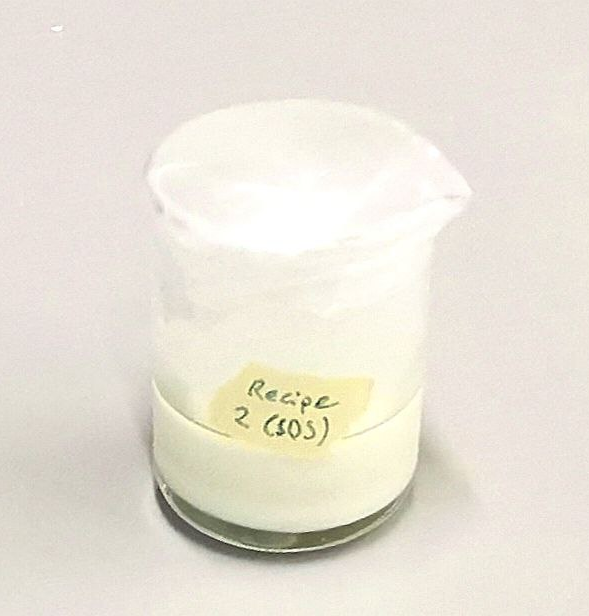
\includegraphics[width=.99\textwidth]{Pics/sol-aq.png}
		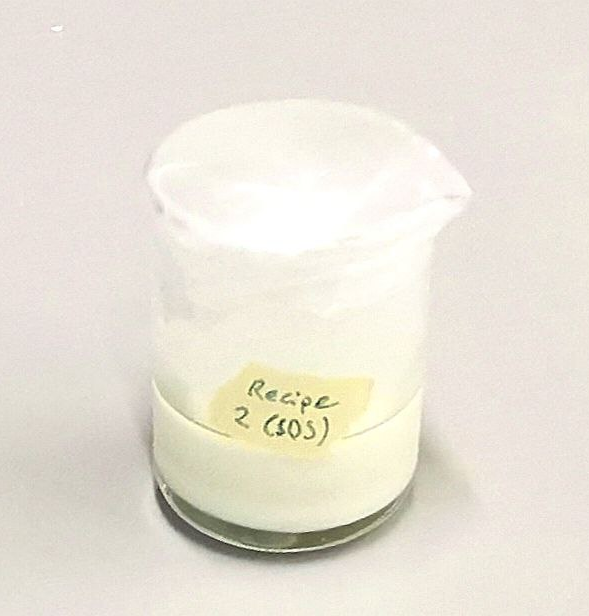
\includegraphics[height=0.8\textwidth]{Pics/sol-aq.png}
		\label{fig:sol-aq}
		\caption{Aquatic solution}
	\end{subfigure}
	\begin{subfigure}{0.49\textwidth}
		\centering
		%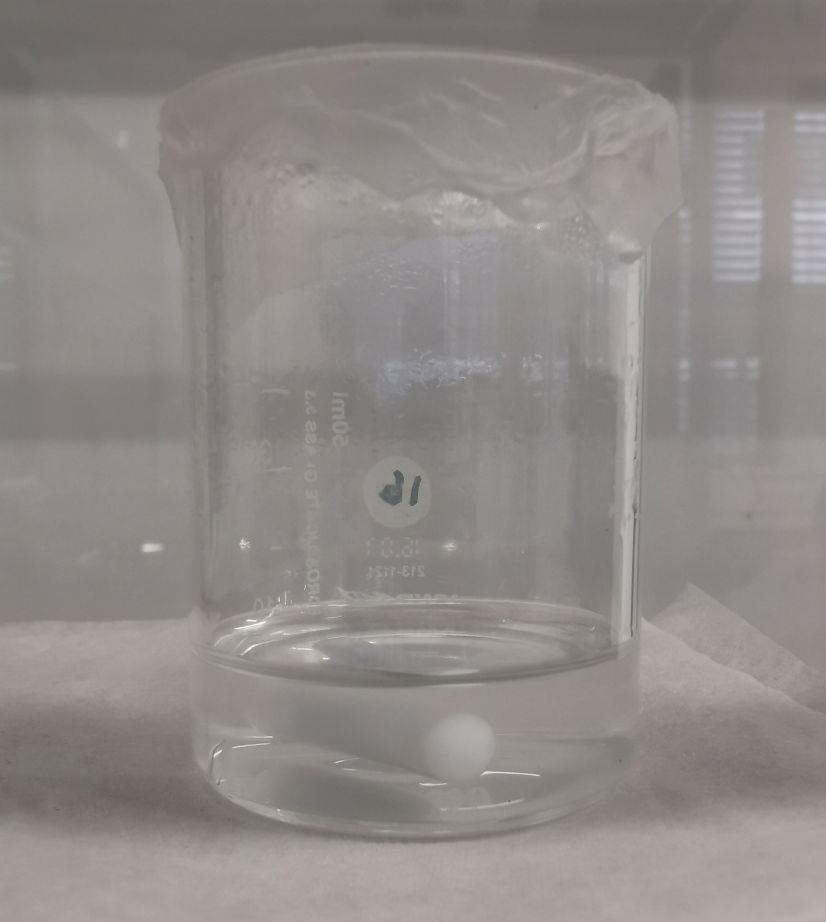
\includegraphics[width=.99\textwidth]{Pics/sol-bu.png}
		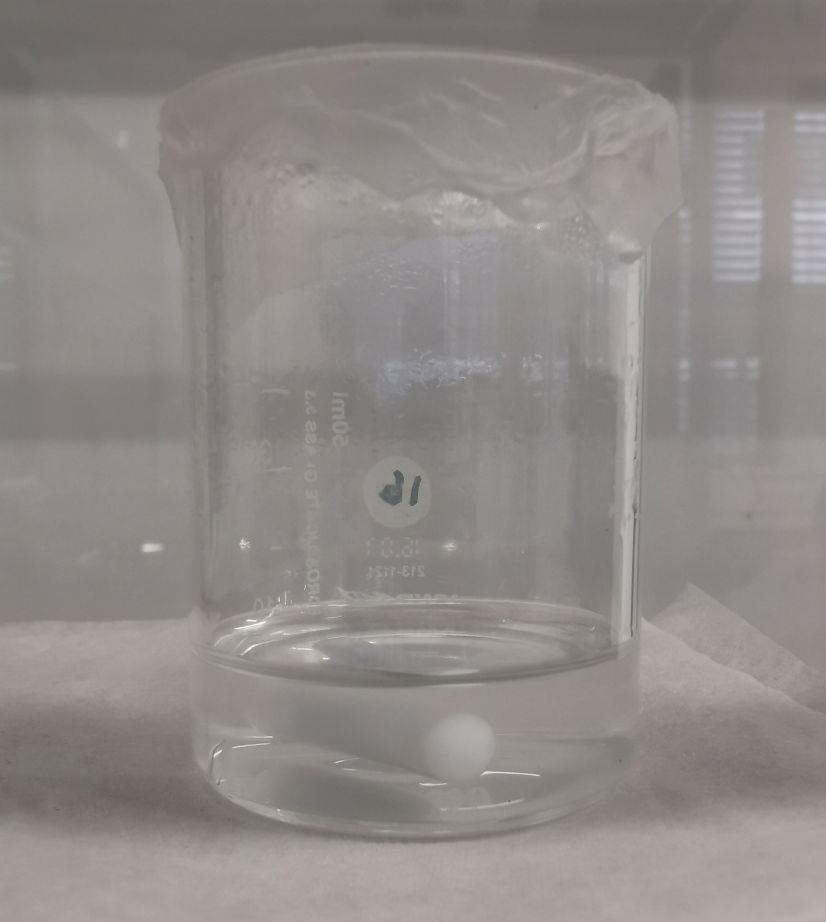
\includegraphics[height=0.8\textwidth]{Pics/sol-bu.png}
		\label{fig:sol-bu}
		\caption{Buthanolic solution}
	\end{subfigure}
	\label{fig:sol}
	\caption{Aquatic and buthanolic solution in beaker glass with magnetic stirring bars sealed with Parafilm} 
\end{figure}
%\fi

%%%%%%%%%%%%%%%%%%%%%%%%%%%%%%%%%%%%%%%%%%%%%%%%%%%%%%
\subsubsection{Aquatic solution}
%\me{The procedure for the aquatic solution is as follows:}
\gls{zrpro} was added to \gls{acac} while stirring and in a separate vessel \gls{water} (including any optional additives such as \gls{sds}, \gls{hcl}, \gls{h2so4} or \gls{naoh}) was added to \gls{ipo} and both were stirred for one hour. 
The \gls{water}-\gls{ipo} mixture was added to the other solution and stirred over night. 
The exact volumes can be taken from table~\ref{tab:rec1}.
\begin{table}[h]
	\centering
	\caption{Compositions of different aquatic solutions}
	\label{tab:rec1}
	\begin{tabular}{llllllll}
		\hline
		recipe				&1		&2		&3		&4		&5		&6		&7\\
%		\hline
%		conc. [a.u.]	&1		&1.7	&2.6	&3.5	&4.4	\\
		\hline
		\gls{zrpro} [\ml{}]	&8		&8		&8		&8		&8		&8		&8\\
		\gls{acac}  [\ml{}]	&8		&8		&8		&8		&8		&8		&8\\
		\gls{ipo}   [\ml{}]	&2		&2		&2		&2		&2		&2		&2\\
		\gls{water} [\ml{}]	&2.6	&2.6	&2.5	&2~		&2		&2		&2\\
		\gls{sds}   [\mg{}]	&-		&5.9	&-		&-		&-		&-		&-\\
		\gls{hcl}   [\ml{}]	&-		&-		&-		&-		&0.5	&-		&-\\
		\gls{h2so4} [\ml{}]	&-		&-		&-		&-		&-		&0.5	&-\\
		\gls{naoh}  [\ml{}] &-		&-		&-		&-		&-		&-		&0.5\\
		\hline
	\end{tabular}
\end{table}
%
%%%%%%%%%%%%%%%%%%%%%%%%%%%%%%%%%%%%%%%%%%%%%%%%%%%%%%
\subsubsection{Buthanolic solution}
\label{sec:sol}
Five different concentration were prepared. 
%The first solution \td{(standard concentration/ one fold/ 1F)} 
%followed the recipe loosely, which is described by Hu et al. \cite{Hu2016}.
%In order to obtain thicker \gls{zro} layers the \gls{zrpro} concentration in the starting solution was raised.
The \gls{1f} 
was closest to the recipe proposed by Hu et. al. \cite{Hu2016}. 
The other four solutions (\gls{2f}, \gls{3f}, \gls{4f}, \gls{5f}) were similar with higher concentrations of \gls{zrpro} (see table \ref{tab:rec2}).
%%%%%%%%%%%%%%%%%%%%%%%%%%%%%%%%%%%%%%%%

\begin{table}[h]
	\centering
	\caption{}
	\label{tab:rec2}
	\begin{tabular}{rlllll}
		\hline
				&1F		&2F		&3F		&4F		&5F		\\
		\hline
%		conc. [a.u.]	&1		&1.7	&2.6	&3.5	&4.4	\\
%		\hline
		\gls{buoh} [\ml{}]		&4.95	&4.9	&4.85	&4.8	&4.75	\\
		\gls{zrpro} [\ml{}]	&0.05	&0.1	&0.15	&0.2	&0.25	\\
		\gls{acac} [\ml{}]		&0.0125	&0.025	&0.0375	&0.05	&0.0625	\\
		\gls{ipo}/\gls{acoh} [\ml{}]		&2		&2		&2		&2		&2		\\
		\hline
	\end{tabular}
\end{table}

\iffalse
The procedure for obtaining the \gls{1f} solution will be explained in detail: \td{maybe just keep it general}
%
%was closely on the basis of ref \cite{Hu2016}. 
%The standard concentration will be described first and then the differences of higher concentrated solutions:
\ml{4.9} of solvent (\gls{buoh}) are put into a beaker glass (or similar, preferably with an air-tight cap) with a stirrer. 
\ml{0.1} of \gls{zrpro} are added while stirring.  
After 10 to 15 minutes \ml{0.05} (\ds{approximately }one mole equivalent of \gls{zrpro}) chelating agent (\gls{acac}) were added and stirred for another \minutes{10 to 15}. 
Finally, \ml{1} of stabilisation solvent (\gls{ipo} or \gls{acoh}) was added to the mixture and stirred for additional 20-30 minutes. 
\fi
%%%%%%%%%%%%%%%%%%%%%%%%%%%%%%%%%%%%%%%%
The solvent (\gls{buoh}) was put into a beaker glass (or similar, preferably with an air-tight cap) with a stirrer and \gls{zrpro} was added while stirring.  
After stirring \minutes{\ds{10 to }15} one mole equivalent chelating agent (\gls{acac}) was added and stirred for another \minutes{\ds{10 to }15}. 
Finally, the stabilisation solvent\cite{Hu2016} (\gls{ipo} or \gls{acoh}) was added to the mixture and stirred for additional \minutes{\ds{20-}30}. 
%%%%%%%%%%%%%%%%%%%%%%%%%%%%%%%%%%%%%%%%
In order to make a \gls{2f} solution, the volume of \gls{zrpro} and \gls{acac} was doubled and \gls{buoh} was decreased by the volume of \gls{zrpro}. 
%The real concentration of a \gls{2f} solution is not double of the original, though, but rather 1.7 fold because volume of \gls{ipo} is kept constant.

\subsection{Doctor blading}
\label{sec:DB}
%{The temperature of the heating plate is set to 200 $^o$C.
%The temperature of the vacuum plate is set and waited until reached.
%The velocity of the \gls{db} blade is set and it is %\td{a mini test run is performed.} 
%tested if the sample can be retained in place by the under-pressure.
%The blade is put in position. 
%The sample is placed on the vacuum plate and the vacuum is switched on. }
After setting the heating plate temperature, the vacuum plate temperature (see figure \ref{fig:eric}) and the \gls{db} velocity, the \gls{db} blade is put into position and the sample placed on the vacuum plate. 
The vacuum is switched on and the blade is sent over the sample without liquid to see if it is held in position.
\ul{100} of solution is applied with an 10-\ul{1000} pipette and the blade moves over the sample distributing the liquid evenly. %\td{the doctor blading} is started immediately. 
After evaporation of the solution, the vacuum is turned off, the 'blade pusher' put into initial position, the blade removed and excess solution removed with a wipe. 
The small metal plate is transferred to the hot heating plate and rests on there for 3-\minutes{5}. 
The process is repeated as wished. 
\begin{figure}
	\centering
	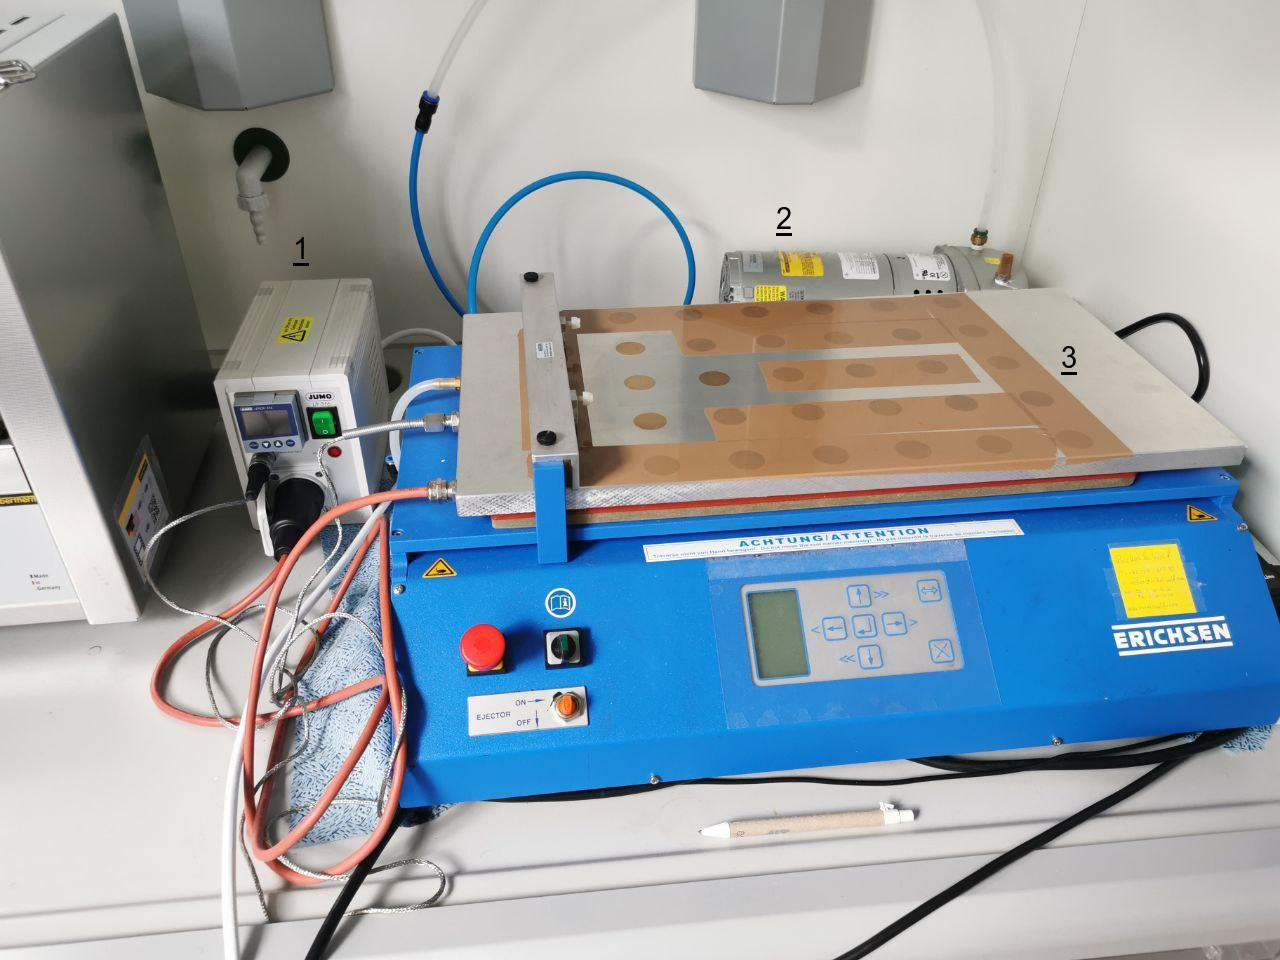
\includegraphics[width=.8\textwidth]{Pics/erichsen1.png}
	%\caption{(3) Erichsen Coatmaster 510 with (2) vacuum pump in the background and (1) temperature regulator on the left.}
	\caption{
		(1) Temperature regulator on the left,
		(2) vacuum pump in the background and 
		(3) Erichsen Coatmaster 510 with heatable vacuum plate.
		The majority of the suction areas is sealed with tape to increase the under pressure at the remaining ones.
		\todo{add picture with blade}
	}
	\label{fig:eric}
\end{figure}

\subsection{Calcination}
A LabTech EH45 C heating plate and a Naberterm L B410 furnace were used to calcinate the doctor bladed samples. 
%The heating plate heated with a steady rate of \td{\oc{5}/\minutes{}}.
%The heating plate can hold temperature for a certain amount of time, but doesn't have conifgurable heating rates.
The heating late can hold temperature for a certain amount of time, but heated with a fixed rate of circa \oc{10}/\minutes{}.
In order to achieve a lower overall heating rate several temperature ramps and plateaus were alternated (see table~\ref{tab:labtech}).
This procedure will be called HP1 from now on, which stands for heating plate procedure.
The HP1 procedure was optimized for the available hardware by a colleague working on the project prior to the author.

\begin{table}[h]
	\centering
	\begin{tabular}{rl ll ll ll ll ll ll }%ll ll ll ll ll ll ll}
%			&temp [\oc]	&time/rate &temp [\oc]	&time/rate	&temp [\oc]\\
		HP1		&&&&&&&&&&&&&\\
		\hline
		T [\oc{}]	    &80		&100	&150	&160	&170 	&180	&190	&200	&250	&300	&350	&400	\\
		t [\minutes{}]	&10 	&10		&5 		&5 		&5 		&5 &5 &10 &10 &10 &10 &60 \\
		\hline
	\end{tabular}
	\caption{Time the temperature was held constant at certain temperatures on the heating plate}
	\label{tab:labtech}
\end{table}
%
The NT1 heating program was used to mimic the HP1 heating procedure in the Naberterm furnace. 
NT2 is an simplification of NT1 and programs NT3-NT6 are the same as NT2 with altered heating rate and partly increased calcination temperature T$_{\textrm{Cal}}$ (NT5).
NT2-NT6 had only 2 variables (heating rate and calcination temperature) instead of 4 (three different heating rates and calcination temperature). 
%where the \td{calcination time} was held constant.
%The time at maximum temperature was held constant over all heating procedures.
All heating programs were held at the calcination temperature for one hour.
In figure \ref{fig:heat} the different heating curves are depicted. 
%
%
\begin{table}[h]
	\centering
	\begin{tabular}{rl ll ll}% ll ll ll ll }%ll ll ll ll ll ll ll}
%			&temp [\oc]	&time/rate &temp [\oc]	&time/rate	&temp [\oc]\\
%		HP1		&&&&&\\%&&&&&&&&\\
%		\hline
%		T [\oc{}]				&80		&150	&200	&400	&400 	\\
%		$\theta$ [\oc{}/\minutes{}]	&10 	&10		&5 		&5		& 		\\
		\hline\hline
		Name	&80-150\oc{} [\oc{}/\minutes{}]	&150-200\oc{} [\oc{}/\minutes{}]	&200\oc{}-T$_{\textrm{Cal}}$ [\oc{}/\minutes{}]	&T$_{\textrm{Cal}}$ [\oc{}] &t$_{\textrm{Cal}}$ [\minutes{}]	\\
		\hline
		NT1		&2					&1					&2				&400	&60  \\
		NT2		&2					&2					&2				&400	&60  \\
		NT3		&3					&3					&3				&400	&60  \\
		NT4		&4					&4					&4				&400	&60  \\
		NT5		&4					&4					&4				&500	&60  \\
		NT6		&1					&1					&1				&400	&60  \\
%		NT7		&max				&max				&max			&600	&60  \\
		\hline\hline
	\end{tabular}
	\caption{Heating rates and calcination temperature holding times. }
	\label{tab:nt}
\end{table}

\begin{figure}
	\centering
	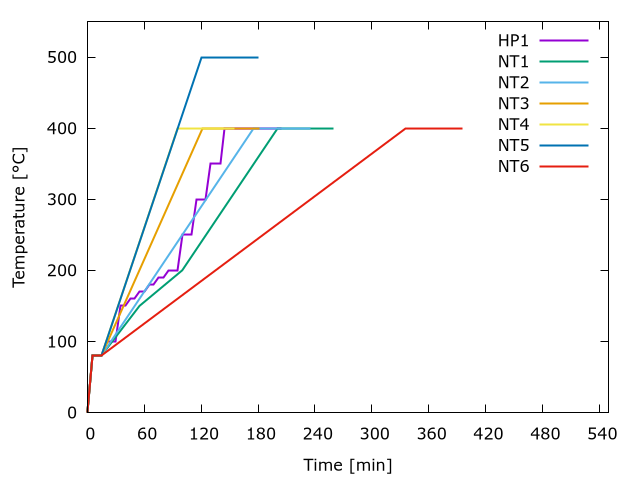
\includegraphics[width=.7\textwidth]{../Data/Graphs/hp1.png}
	\caption{Different heatings curves}
	\label{fig:heat}
\end{figure}

\subsection{Characterisation}
%\url{https://link.springer.com/content/pdf/10.1186/2228-5326-3-8.pdf}
All scanning electron microscopy images were taken with a Zeiss Supra 40. 
%
Infrared spectra were recorded with a Bruker Vertex 70 spectrometer. 
%
Diffraction spectra were obtained with a Thermo Scientific ARL Equinox 100 X-Ray Diffractometer. 
%\subsubsection{SEM}
%AllZeiss Supra 40
%\subsubsection{Infrared}
%Bruker Vertex 70
%\subsubsection{X-Ray Diffraction}
%The sample was placed in a way such that it absorbed half of the beam. 
All spectra were taken at \SI{5}{\degree} incident angle and compared to the internal database.
%Thermo Scientific ARL Equinox 100 X-Ray Diffractometer\\
%\subsubsection{Current-Voltage Curve}
The current-voltage curves were measeured with Agilent 4156C Precision Semiconductor Parameter Analyzer after sputtering Aluminium contacts through a mask with a Leybold UNIVEX450C Sputter System.
%\td{Sputtering Machine} assisted by \td{Leybold Univex 450 C} for the vacuum. In this work, the Al layers were deposited with the Leybold UNIV
\begin{figure}
	\centering
	\begin{subfigure}{0.48\textwidth}
		\centering
		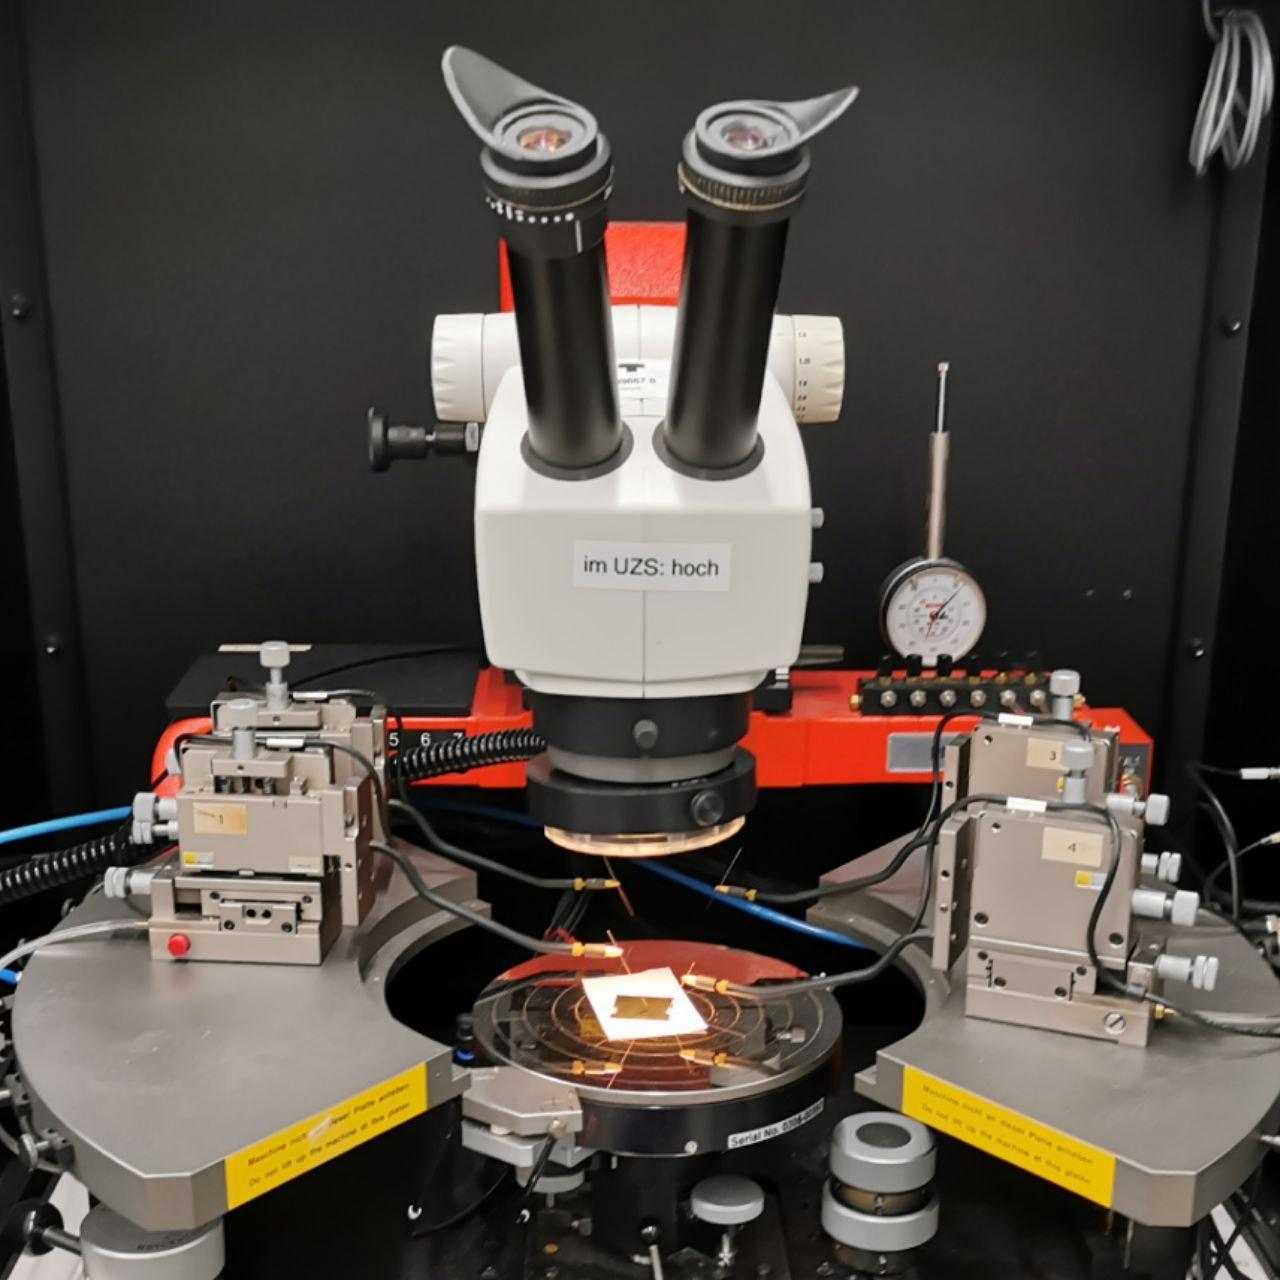
\includegraphics[width=.9\textwidth]{Pics/i-v.png}
		\label{fig:iv-agilent}
		\caption{peripherals}
	\end{subfigure}
	\begin{subfigure}{0.48\textwidth}
		\centering
		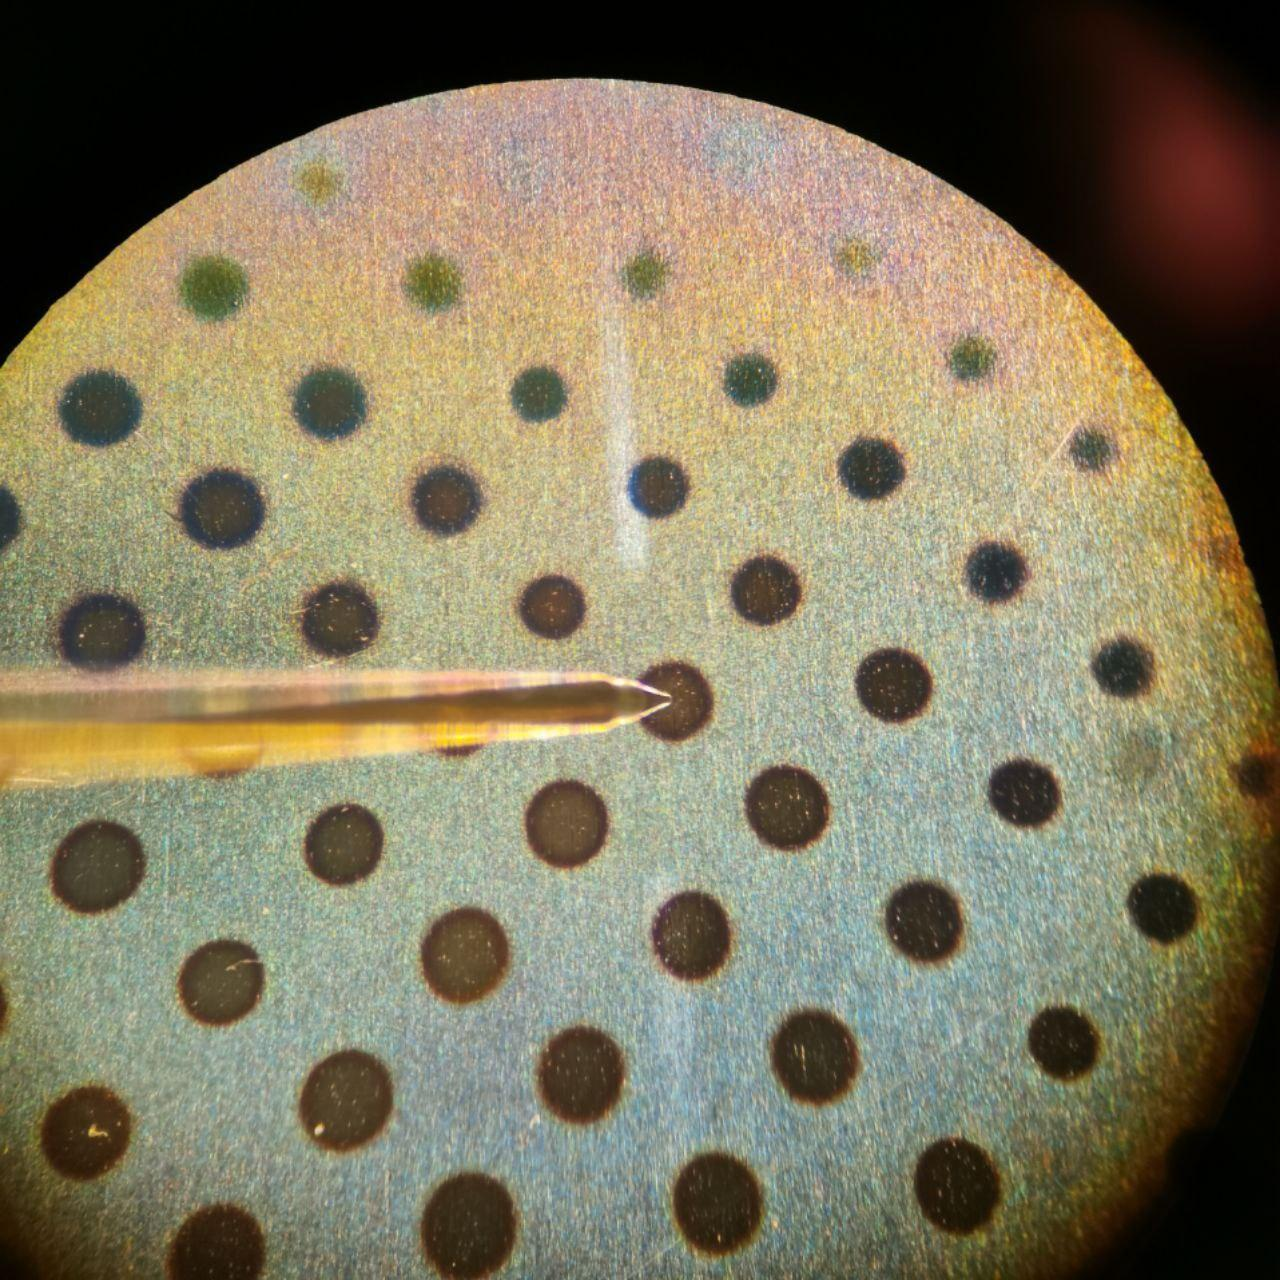
\includegraphics[width=.9\textwidth]{Pics/i-v-micro.png}
		\label{fig:iv-micro}
		\caption{View through the microscope}
	\end{subfigure}
	\label{fig:iv}
	\caption{I-V curve abnehm aperature and sicht durch das micro scope.}
\end{figure}

\subsection{Finding base process}
After a fitting recipe was found, the process to produce an accaptable layer was untersucht. 
There were many variables which had to be taken into account. 
The damals current procedure produced clear and continuous films, but was plagued from unhomogenities due to drying stains. 
Using a heat gunn the drying stain can be surcumvented (umgangen), but the results were unreproduceable. 
The glass unterlage was therefore exchanged with a metal plate which allowed both to hold the sample via underpressure and heat it to a certain temperature.
The bounds fore the process were then explored. 
Especially the doctor blading velocity.




\iffalse
\subsection{EMMA Propagation}
\begin{table}
	\centering
	\begin{tabular}{ccccccc}
		\hline
		\hline
conc	&layers	&vDOC	&TDOC	&vCal	&Tcal	&	\\
		\hline
1	&10	&5	&20	&120	&400	&\\
1	&4	&0.1	&20	&120	&500	&\\
5	&10	&0.1	&20	&120	&500	&\\
5	&4	&5	&20	&480	&400	&\\
1	&5	&5	&80	&120	&500	&\\
1	&10	&1	&80	&480	&400	&\\
5	&5	&1	&80	&120	&400	&\\
5	&10	&5	&80	&480	&500	&\\
2	&8	&0.5	&40	&360	&470	&\\
2	&6	&2	&40	&360	&430	&\\
		\hline
%4	&12	&-	&-	&-	&-&\\
1	&4	&12	&70	&120	&500	&\\
1	&9	&18	&80	&240	&400	&\\
%2	&5	&18	&70	&-	&-		&\\
4	&6	&14	&60	&240	&500	&\\
4	&6	&14	&60	&240	&500	&\\
4	&6	&14	&60	&240	&500	&\\
		\hline
2	&10	&20	&40	&120	&500	&6113\\
3	&8	&18	&70	&1080	&300	&2850\\
3	&6	&10	&50	&1080	&400	&5526	\\
%3	&10	&14	&50	&600	&500	&-7374	\\
3	&10	&16	&80	&120	&500	&6554	\\
4	&6	&16	&80	&1080	&300	&2947	\\
3	&12	&12	&80	&840	&500	&8318	\\
3	&10	&14	&50	&600	&500	&7374	\\
5	&6	&10	&60	&1080	&400	&5648	\\
5	&10	&20	&60	&360	&300	&3956	\\
5	&12	&14	&60	&1080	&300	&2700	\\
		\hline
%2	&2	&10	&40	&600	&300	&-7201	\\
2	&4	&10	&80	&1080	&300	&6101	\\
%2	&4	&10	&40	&600	&300	&-7201	\\
2	&4	&10	&40	&600	&300	&7201	\\
3	&4	&12	&60	&600	&300	&1462	\\
4	&4	&10	&80	&1080	&300	&2883	\\
5	&12	&20	&70	&600	&300	&1680	\\
		\hline
2	&4	&10	&40	&120	&300	&1	\\
2	&4	&10	&40	&120	&500	&6001	\\
3	&4	&10	&40	&120	&500	&6102	\\
5	&4	&10	&80	&1080	&300	&2884	\\
5	&12	&20	&60	&120	&300	&360	\\
		\hline
3	&4	&10	&40	&600	&400	&4202	\\
2	&6	&20	&40	&120	&500	&6105	\\
%4	&4	&14	&80	&1080	&300	&-2923	\\
5	&12	&14	&60	&600	&300	&1500	\\
3	&6	&14	&60	&600	&300	&1486	\\
4	&4	&14	&80	&1080	&300	&2923	\\
		\hline
4	&8	&18	&80	&1080	&300	&2971	\\
3	&8	&10	&50	&1080	&300	&2530	\\
2	&12	&16	&40	&120	&400	&3077	\\
2	&10	&18	&60	&1080	&300	&2733	\\
4	&10	&10	&50	&1080	&300	&2535	\\
		\hline
		\hline
	\end{tabular}
	\caption{}
	\label{tab:emma}
\end{table}
\fi


\section{Evaluation and Computational Details}
\subsection{Evaluation of Samples}
\label{sec:eval}
For every I-V curve (aluminium dot) the gradient $g$ at $V=0$ is calculated by taking 5 points after the origin and 5 points before the origin, averaging their V and I values and calculating i
\begin{equation}
	g = \frac{I_{n+1} - I_n}{V_{n+1} - V_n}.
\end{equation}
As a measure of conductance a distance D from an ideal non-conducting case. The average of the negative base 10 logarithm subtracted from an ideal non-conducting gradient of $10^{-13}$ 
\begin{equation}
	D = \sum_i^N \frac{ -log_{10}(g_i) - 13}{N}
	\label{eq:D}
\end{equation}
Another measure is the density of shorted species $\rho_{s}$ is calculated in following way:
\begin{equation}
	s_i = \begin{cases}
	1 &\text{if} \quad -log(g_i) < 5 \\
	0 &\text{if} \quad -log(g_i) \geq 5 \\
	\end{cases}
\end{equation}
\begin{equation}
	\rho_s = \sum_i^N \frac{s_i}{N}
	\label{eq:rho}
\end{equation}
Other estimates of the conductance are the averages:
\begin{equation}
	G_1 = log \left( \sum_i^N \frac{g_i}{N} \right)
\end{equation}

\begin{equation}
	G_2 =  \sum_i^N \frac{log(g_i)}{N}
\end{equation}

\subsection{Sample Selection}
\label{sec:ss}
An evolutionary approach was chosen, namely a multi-objective Particle Swarm Optimization (PSO) with a multi-response
Multivariate Adaptive Regression Splines (MARS) model\cite{Villanova2010,Kennedy1995,Breiman1997,Carta2011}.
%
"PSO is a population based heuristic inspired by the flocking behavior of birds. 
To simulate the behavior of a swarm, each bird (or particle) is allowed to fly towards the optimum solution."\cite{Villanova2010}
%
Initially the input parameters (independent variables), their boundaries and number of equidistant levels for each parameter are declared (see table \ref{tab:input}).
Next, the output variables (dependant variables), their weights in the objective function (the function which should be optimized) are specified and if they should be minimized or maximized is noted.
%
%An initial population of particles, i.e. experiments with certain parameters, is chosen out of the population space (space spanned by all possible combinations of input parameters), 
\begin{table}[htb]
	\centering
	\begin{tabular}{cc cc cc}
		\hline
		Zr(PrO)$_4$ conc. [21 g/L]	&layers	&$T_{DB}$[\oc{}]	&$v_{DB}$[\mm{}/\s{}]	&$T_{cal}$[\oc{}]	&$v_{cal}$[\oc{}/\h{}]	\\
		\hline
		2				&4		&40					&10				&300				&120	\\
		3				&6		&50					&12				&400				&360	\\
		4				&8		&60					&14				&500				&600	\\
		5				&10		&70					&16				&					&840	\\
						&12		&80					&18				&					&1080	\\
						&		&					&20				&					&		\\
		\hline
	\end{tabular}
	\caption{Discrete levels of each input parameter \td{are concentrations correct?}}
	\label{tab:input}
\end{table}

The first step is to select an initial population (ensemble of experiments), which is chosen randomly from the population space. 
The samples are made, measured and evaluated according to section \ref{sec:exp} and the distance $D$ (see eq. \ref{eq:D}), $\rho_s$ (see eq. \ref{eq:rho}), $n_{layers}$ (numbers of layers) and $v_{cal}$ (heating rate of calcination process in \oc{}/\minutes{}) are supplied to the program. 
The program uses this data to estimate a response for each output variable (and to choose a fraction of the initial population which is allowed to propagate).
The response variables for the entire population space is calculated. 
The current population - each of the particles independently - moves towards the optimum solution.
The population for the next time step is outputted and the experiments are again executed, measured and evaluated.

\subsection{EMMA Propagation}
\begin{table}[htb]
	\centering
	\begin{tabular}{ccccccc}
		\hline
		\hline
conc	&layers	&vDOC	&TDOC	&vCal	&Tcal	&	\\
		\hline
1	&10	&5	&20	&120	&400	&\\
1	&4	&0.1	&20	&120	&500	&\\
5	&10	&0.1	&20	&120	&500	&\\
5	&4	&5	&20	&480	&400	&\\
1	&5	&5	&80	&120	&500	&\\
1	&10	&1	&80	&480	&400	&\\
5	&5	&1	&80	&120	&400	&\\
5	&10	&5	&80	&480	&500	&\\
2	&8	&0.5	&40	&360	&470	&\\
2	&6	&2	&40	&360	&430	&\\
		\hline
%4	&12	&-	&-	&-	&-&\\
1	&4	&12	&70	&120	&500	&\\
1	&9	&18	&80	&240	&400	&\\
%2	&5	&18	&70	&-	&-		&\\
4	&6	&14	&60	&240	&500	&\\
4	&6	&14	&60	&240	&500	&\\
4	&6	&14	&60	&240	&500	&\\
		\hline
2	&10	&20	&40	&120	&500	&6113\\
3	&8	&18	&70	&1080	&300	&2850\\
3	&6	&10	&50	&1080	&400	&5526	\\
%3	&10	&14	&50	&600	&500	&-7374	\\
3	&10	&16	&80	&120	&500	&6554	\\
4	&6	&16	&80	&1080	&300	&2947	\\
3	&12	&12	&80	&840	&500	&8318	\\
3	&10	&14	&50	&600	&500	&7374	\\
5	&6	&10	&60	&1080	&400	&5648	\\
5	&10	&20	&60	&360	&300	&3956	\\
5	&12	&14	&60	&1080	&300	&2700	\\
		\hline
%2	&2	&10	&40	&600	&300	&-7201	\\
2	&4	&10	&80	&1080	&300	&6101	\\
%2	&4	&10	&40	&600	&300	&-7201	\\
2	&4	&10	&40	&600	&300	&7201	\\
3	&4	&12	&60	&600	&300	&1462	\\
4	&4	&10	&80	&1080	&300	&2883	\\
5	&12	&20	&70	&600	&300	&1680	\\
		\hline
2	&4	&10	&40	&120	&300	&1	\\
2	&4	&10	&40	&120	&500	&6001	\\
3	&4	&10	&40	&120	&500	&6102	\\
5	&4	&10	&80	&1080	&300	&2884	\\
5	&12	&20	&60	&120	&300	&360	\\
		\hline
3	&4	&10	&40	&600	&400	&4202	\\
2	&6	&20	&40	&120	&500	&6105	\\
%4	&4	&14	&80	&1080	&300	&-2923	\\
5	&12	&14	&60	&600	&300	&1500	\\
3	&6	&14	&60	&600	&300	&1486	\\
4	&4	&14	&80	&1080	&300	&2923	\\
		\hline
4	&8	&18	&80	&1080	&300	&2971	\\
3	&8	&10	&50	&1080	&300	&2530	\\
2	&12	&16	&40	&120	&400	&3077	\\
2	&10	&18	&60	&1080	&300	&2733	\\
4	&10	&10	&50	&1080	&300	&2535	\\
		\hline
		\hline
	\end{tabular}
	\caption{}
	\label{tab:emma}
\end{table}



\subsection{Fitting via Machine Learning}
\td{scarce data may lead to overfitting\cite{Lecun1995conv}}\\
Python and sci-kit learn \td{cite} was used to implement a linear fit model, and SVR with the kernels polynomial, rbf and sigmoid. 
The space of hyper parameters C, the degree (in case of polynomial), epsilon and gamma was scaned. 


\clearpage
\section{Results and Discussion}
\todo{Following stirring times (in minutes) were tested and didn't have an influence on stability of the solution: 10-10-20, 10-10-45, 30-30-180.}
The space seems to be too big for the small sample size.
Look at relation of space size and sample size here and in Hu2016.

Would be easier to fit with single factor at a time variation or latin hyper cuber?
Would it also be easier for PSO or ML to find fitting function?
Every output var is independent of each other, so $v_{cal}$ can act as test 

plot predictions from EMMA and ML.
the data has a lot of error, but because the production process takes so long nad the limited time and the chosen optimisation method, the experiments weren't weiderholt
how much variance is in data? 


\subsection{XRD}

\begin{figure}
	\centering
	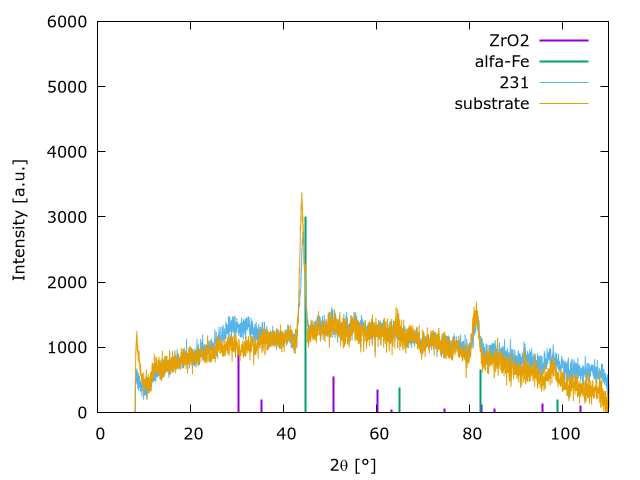
\includegraphics[width=\picwidth]{Pics/xrd.png}
	\caption{XRD spectra}
	\label{fig:xrd}
\end{figure}
\section{Outlook}

Making of the solution for the sol-gel process:
For a single concentrated solution \ml{0.05} of \gls{zrpro} are added while stirring to \ml{4.95} of \gls{buoh} and stirred for \minutes{15}. 
\ml{0.013} (or one molar equvilent of Zr) of \gls{acac} is added to the stirring solution. 
After another \minutes{15} \ml{1} of acetic acid is added and stirred for \minutes{30} to stabilize the solution up to \h{24}. 

The concentration can be increased up to 5 times being stable for a minimum of \h{4}. 
The sol-gel process produces am homogeneous transparent crystalline zirconia oxide layer. 
homogeneity can be mainly controlled via blade velocity and temperature and layers can be stacked.

It should have been alos verglichen with grid search with comparable size
but most time was used to find a vernuenfig base recipe and process

It is still very human 
Der process is - as it the case with all ML and most fitting processes - is very abhaengig von hyper parameters, 
In the current work population size, number of generations, and most importantly boundaries (grenzen). 


%\clearpage
\bibliographystyle{ieeetr}
\bibliography{int}
\end{document}
